\documentclass[11pt,twoside,a4paper]{scrartcl}
	\usepackage[english]{babel}
	\usepackage{amsmath}
	\usepackage{amsthm}
	\usepackage{amssymb}
	\usepackage{hyperref}
	\usepackage{graphicx}
	\usepackage{listings}
	\usepackage{color}

	\usepackage[nameinlink,capitalise]{cleveref}

	%Link colors
	\usepackage{xcolor}
	\definecolor{dark-red}{rgb}{0.4,0.15,0.15}
	\definecolor{dark-blue}{rgb}{0.15,0.15,0.4}
	\definecolor{medium-blue}{rgb}{0,0,0.5}
	\definecolor{bg}{rgb}{0.95,0.95,0.95} % Needed for listing background
	\hypersetup{%
		colorlinks, linkcolor={dark-blue},
		citecolor={dark-blue}, urlcolor={medium-blue}
	}

	\definecolor{mycomment}{rgb}{0.3,0.7,0.8}
	\definecolor{mygray}{rgb}{0.5,0.5,0.5}
	\definecolor{lightgray}{rgb}{0.95,0.95,0.95}
	\definecolor{mymauve}{rgb}{0.58,0,0.82}

	\lstset{%
	  backgroundcolor=\color{lightgray},
	  basicstyle=\footnotesize,
	  breakatwhitespace=false,
	  breaklines=true,
	  captionpos=b,
	  commentstyle=\color{mycomment},
	  escapeinside={\%*}{*)},
	  extendedchars=true,
	  keepspaces=true,
	  keywordstyle=\color{black}\bfseries,
	  language=matlab,
	  numbers=left,
	  numbersep=5pt,
	  numberstyle=\tiny\color{mygray},
	  rulecolor=\color{black},
	  showspaces=false,
	  showstringspaces=false,
	  showtabs=false,
	  stringstyle=\color{mymauve},
	  tabsize=2,
	  title=\lstname
	}

	%Pseudocode
	\usepackage{algorithm}
	\usepackage[noend]{algpseudocode}

	% Euro symbol
	\usepackage[official]{eurosym}

	% SI-units
	\usepackage{siunitx}

	% Circuit drawing
	\usepackage[siunitx]{circuitikz}

	% Code listings
	\usepackage[section]{minted}
	\newmintedfile[cfile]{c}{%
		frame=leftline,
		linenos=true,
		tabsize=4,
		bgcolor=bg
	}

	% Todos
	\usepackage{todonotes}

	\title{A Fiber Tap Proof of Concept}
	\subtitle{Tapping Communications on the Cheap}
	\author{%
		Eddie Schoute, 4101790\\
		Alex van Rijs, ???
	}

\begin{document}
\maketitle

\begin{abstract}
	\noindent Network security is a very important concept in today's information society.
	With the heavy reliance on data communications, comes also a responsibility for its security.
	While fiber cables are an improvement over traditional copper with respect to tapping,
	it is still very possible to tap these cables as we will show in this paper.
	We will give a proof of concept of tapping fiber communications ``on the cheap'',
	using less than \euro{}$20$ in hardware materials.
	As such we recommend that confidential data communication needs to be encrypted,
	even when using fiber optic cables.
\end{abstract}

\section{Introduction}
	%Subject introduction
	Terabytes of data are being exchanged over fiber optic cables every day and user rely on their security.
	As can be shown with the recent controversy surrounding the tapping of Google and Yahoo network infrastructure~\cite{googleyahootap},
	the pure physical layer of communications is still assumed to be secure.

	%Research question and contributions
	While it is better known that copper taps are easy to install, fiber optic communications are harder to tap.
	In this paper we will investigate the possible ways an intruder may use to tap fiber optic links.
	We we also look into bringing these methods into practice, by supplying a proof of concept implementation.

\section{Design}
	% Some background research and interesting stuff that we used

\section{Proof of Concept}
	For the proof of concept we discern three parties, the sender, receiver and tapper.
	The sender and receiver are legitimate communication parties,
	while the tapper tries to gain access to the communications between them.
	For the proof of concept we used Arduino boards for simple prototyping and some other hardware
	that we will discuss in later sections.
	First we set up a fiber optic communication link between sender and receiver,
	after which we installed the tapper.

	\subsection{Fiber Communication}
		At first we tried to set up a communication using two Arduinos, an LED with a wavelength of about \SI{650}{\nano\meter},
		a fiber cable, a lens and a photoresistor.
		We immediately noticed that simply shining the LED into the cable would not work,
		because not enough light enters the cable using this method.
		When using a lens to focus the light on the cable entrance,
		the results were better but still not satisfactory.
		Only after consulting with the Optics department did we give up on using this method
		and ordered a fiber communication kit.

		The kit included a transmitter at \SI{660}{\nano\meter}, receiver, a fiber cable with connectors and some other materials we did not use.
		The adjoining data sheet describes a circuit for a simple \SI{40}{\kilo Bd} communication link,
		which we used for building a basic communication link~\cite[p.15]{avagokit},
		see \cref{fig:transmitter}.
		Initially we planned to have an input resistance of \SI{500}{\ohm} instead of \SI{100}{\ohm},
		but we noticed that the light source has a higher intensity with lower input resistance.
		With more input power it easier to tap the cable, so we opted for a lower resistance.
		The output receiver was built exactly as specified in the data sheet.

		\begin{figure}
			\centering
			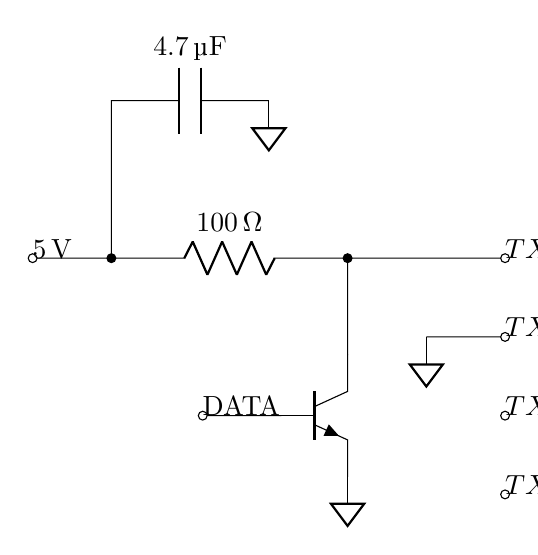
\begin{tikzpicture}
				\draw
				(0,5) node[ocirc] {\SI{5}{\volt}}
				to (1,5) node[circ] (input) {}
				to ++(0,2)
				to[C, l={\SI{4.7}{\micro\farad}}] ++(2,0)
				node[sground] {}

				(input) to[R, l={\SI{100}{\ohm}}] ++(3,0) node[circ] (transmitter) {}
				++(0,-2) node[npn] (npn) {}
				(transmitter) to (npn.collector) {}

				(npn.base) to ++(-1,0) node[ocirc] {DATA}
				(npn.emitter) node[sground] {}

				(transmitter) to ++(2,0) node[ocirc] (tx1) {$TX_1$}
				++(0,-1) node[ocirc] (tx2) {$TX_2$}
				to ++(-1,0) node[sground] {}
				(tx2) ++(0,-1) node[ocirc] {$TX_3$}
				++(0,-1) node[ocirc] {$TX_4$}
				;
			\end{tikzpicture}
			\caption{Circuit of the transmitter}
			\label{fig:transmitter}
		\end{figure}

		During this process we also investigated methods for data transfer and concluded that Manchester coding was simple but effective.
		At first we started to implement this ourselves, but encountered issues regarding timing and synchronization.
		Luckily we found a library that provides Manchester coding for Arduino~\cite{manchestercoding}.
		Using the material we have so far we coded a transmitter and receiver, which have been appended in~\cref{lst:transmitterCode,lst:receiverCode}.
		In the next section we will discuss the modifications in the tapper code.

	\subsection{Fiber Tap}
		The first step of installing a fiber is removing the isolation.
		The biggest problem in this step is that the cable is very vulnerable and could break.
		We used a knife for the plastic outer layer and sandpaper for the vulnerable inner layer.
		Then by bending the cable a part of the light leaks out,
		because for a portion of the light in the cable the angle of incidence is too small.

		Secondly, we attached a photo sensor to the cable.
		At first we tried using a photo resistor whose operation is very simple,
		the resistance decrease with increasing light intensity.
		This works well for low frequency signals (up to \SI{5}{\hertz}),
		but is insufficient for but the lowest speed data transfers.
		We then switched to a photo transistor with a switching speed of at most \SI{15}{\micro\second}~\cite{phototransistor}.
		This allows a frequency of up to \SI{67}{\kilo\hertz} which is sufficient for our purposes.
		We measured the resistance of the attached transistor when the light was ON and OFF
		at \SI{300}{\kilo\ohm} and over \SI{1}{\mega\ohm} respectively.
		Using this information we built a simple pull-up circuit using a little trial-and-error,
		we came to a final pull-up resistor of \SI{100}{\kilo\ohm}\todo{Check}.
		When reading the ADC input to the Arduino resulted in values of $3 \pm 2$ for ON and between $95 \pm 7$ for OFF.

		Now to interpret the sent Manchester data on the fiber tap we needed to threshold the measurements
		at about $50$ to turn it into a $1$ or $0$.
		The given library does not support analog inputs, so we modified the library to use
		a threshold and an analog input for measuring the input signal.
		The resulting library can be found at~\cite{analogmanchestercoding}.

		For better results and sturdiness we have also constructed a simple container,
		which keeps the cable bended and the photo sensor isolated from external light sources.
		We also found out that printing the results does not take an insignificant amount of time,
		resulting in missed bytes on the tap which is why we buffered the data.
		Using the above components we are successfully able to tap increasing numbers of up to
		$128$ in a row at \SI{300}{Bd}, at which point the Arduino memory limit is reached.

\section{Conclusion}

\bibliographystyle{abbrv}
\bibliography{bibl}

\appendix
	\section{Code Listings}
		\begin{listing}
			\cfile{../transmitter/transmitter.ino}
			\caption{The transmitter code.}
			\label{lst:transmitterCode}
		\end{listing}

		\begin{listing}
			\cfile{../receiver/receiver.ino}
			\caption{The tapper code.
				The only difference with the legitimate receiver is \texttt{setupReceive} instead of \texttt{setupReceiveAnalog}.}
			\label{lst:receiverCode}
		\end{listing}

\end{document}
